\documentclass[aps,prl,twocolumn,superscriptaddress,amsmath,amssymb,reprint]{revtex4-2}
\usepackage{graphicx}
\usepackage{bm}
\usepackage[colorlinks,allcolors=blue]{hyperref}
\newcommand{\Lc}{\mathcal{L}}

\begin{document}

\title{How a mean-field fold emerges from a linear many-body Liouvillian:\\
the exceptional point is pinned by the quantum quasipotential}

\author{[Author list to be completed]}
\date{\today}

\begin{abstract}
Mean-field (MF) theories of driven-dissipative ensembles predict bistability, with branches that terminate at saddle-node folds. Recent work has interpreted these folds as ``Liouvillian exceptional lines'' of coalescing steady states. The exact $N$-body Liouvillian, however, is linear and has a unique steady state. We identify the finite-$N$ object that replaces the fold in a permutation-symmetric Rydberg ensemble, which we solve exactly up to $N=70$. The fold becomes an exceptional point (EP) of two \emph{decaying} modes at complex detuning. One mode is the intrabasin relaxation of the surviving branch, the other the escape from the ghost of the vanished branch. The EP drifts onto the fold algebraically, and its imaginary part vanishes as $e^{-\sigma N}$. We derive $\sigma$ from a quantum Wentzel–Kramers–Brillouin (WKB) theory with no free parameter: $\sigma$ equals the rate function of the excitation-number distribution, evaluated at the MF fold population. Two prerequisites, switching exponents and quasipotentials, are reproduced to within $3\%$ and $6\%$ by the same theory. Gaussian-noise and incoherent reductions fail by up to a factor of five. The prediction for $\sigma$ was registered before testing, then confirmed at two drive strengths not used to construct it, with observed-to-predicted ratios $0.93$–$0.96$.
\end{abstract}

\maketitle

\emph{Introduction.}---Nonlinear MF equations are the standard description of collective open quantum systems. Examples include optical and Rydberg bistability~\cite{Carr2013,Xie2025}, Kerr resonators~\cite{Casteels2017,Minganti2018}, and dissipative phase transitions generally~\cite{Minganti2018,Macieszczak2016}. In MF theory a stable branch ends at a fold, where it merges with a saddle. A body of recent work describes such folds as \emph{Liouvillian exceptional lines}~\cite{Xie2025,SunYi2024}, on which the nonlinear generator has coalescing steady states. Encircling these lines has been used to explain chiral switching between collective steady states~\cite{Xie2025}. The exact generator $\Lc_N$ of $N$ atoms is linear, though. Its zero mode is simple and cannot be defective~\cite{HuBudich2025}, and first-order behavior appears only as an isolated slow eigenvalue that closes exponentially with $N$~\cite{Minganti2018,Casteels2017,Ptaszynski2024,Xiang2026}. Two-mode descriptions of the resulting hysteresis exist~\cite{Krimer2019}. What has been missing is a precise spectral counterpart of the fold, together with a theory that predicts its finite-$N$ structure.

We provide both for the minimal model of a dissipative Rydberg gas. Three results follow. (i) The MF ``exceptional line'' is a fold of fixed points: the Jacobian there has the closed-form, nondefective spectrum $\{0,-\gamma\pm i\Omega/\sqrt2\}$. (ii) In $\Lc_N$ the fold appears as an EP of two specific decaying modes, and we identify both. (iii) The distance of this EP from the real axis is controlled by a quantum WKB rate function, which we compute \emph{a priori} and test against data that played no role in constructing it.

\begin{figure*}[t]
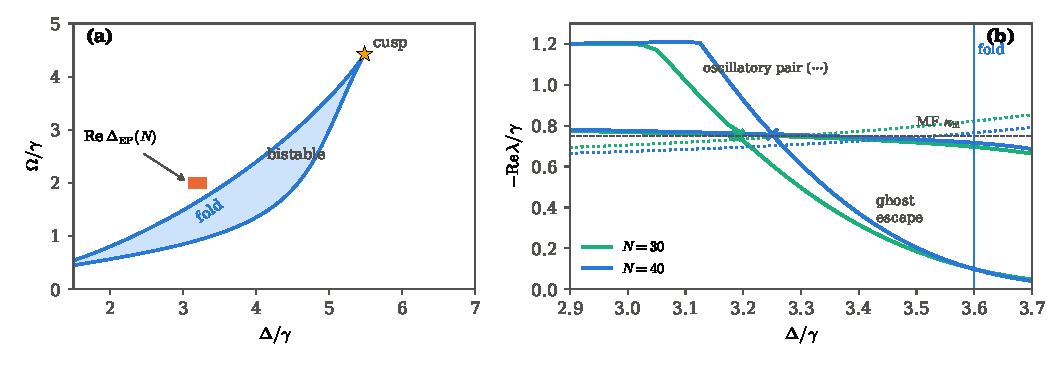
\includegraphics[width=\textwidth]{../figs/rev_fig1.pdf}
\caption{(a) MF bistable wedge (shaded) bounded by fold lines (blue) and terminating at a cusp (star). At $\Omega=2$, ticks mark ${\rm Re}\,\Delta_{\rm EP}(N)$ for $N=20$--$58$; they approach the left fold from outside the wedge. (b) Slowest real modes of the exact $\Lc_N$ near the left fold ($N=30,40$; solid). The ghost-escape branch (falling toward the fold) undergoes an avoided crossing with the high-branch relaxation mode, which stays near the MF value $\kappa_{\rm hi}$ (dashed). Crosses: real part of the exact complex-$\Delta$ EP. Dotted: the oscillatory pair, which is slower than both real modes in part of this window.}
\label{fig:spec}
\end{figure*}

\emph{Model and MF geometry.}---We consider $N$ two-level atoms with uniform interaction $V/N$ and local decay $\hat L_i=\sqrt\gamma\,\hat\sigma^-_i$:
\begin{equation}
\hat H=-\Delta\hat N_e+\Omega\hat J_x+\tfrac{V}{2N}\hat N_e(\hat N_e-1).
\label{eq:H}
\end{equation}
We set $\gamma=1$ and $V=10$. Permutation symmetry reduces $\Lc_N$ to dimension $\binom{N+3}{3}$~\cite{Shammah2018}, which allows sparse shift-invert diagonalization up to $N=70$. In the limit $N\to\infty$, Eq.~\eqref{eq:H} gives Bloch equations with detuning $\Delta-Vn$, where $n=\langle\hat N_e\rangle/N$. The stationary populations solve a cubic, which has three roots inside the wedge of Fig.~\ref{fig:spec}(a). At a fold two roots merge. Eliminating the coherences, the characteristic polynomial of the Bloch Jacobian on the fold reduces exactly to
\begin{equation}
\chi(\lambda)=\lambda\big[(\lambda+1)^2+\Omega^2/2\big].
\label{eq:jac}
\end{equation}
The zero eigenvalue is simple even at the cusp, so no Jordan block appears in the Jacobian. The ``third-order'' structure lives only in the fixed-point equation (a triple root). At the fold, the surviving high branch relaxes with real rate $\kappa_{\rm hi}=0.751$ ($\Omega=2$).

\emph{The exceptional point that replaces the fold.}---Figure~\ref{fig:spec}(b) shows the real part of the slow spectrum of $\Lc_N$ across the left fold. The zero mode is always simple. Two real branches undergo an avoided crossing whose gap closes rapidly with $N$. We locate the EP at complex detuning $\Delta_{\rm EP}(N)$ by Newton iteration on the discriminant of the two eigenvalues. The residual is below $10^{-12}$, and the eigenvector overlap is $1-2\times10^{-14}$ at $N=30$. Encircling $\Delta_{\rm EP}$ in the complex plane exchanges the two branches, the hallmark of a square-root branch point. Because $\Lc$ is linear in $\Delta$, this EP is the analytic continuation of the avoided crossing. The two-level relation ${\rm Im}\,\Delta_{\rm EP}=2g_N/|s_a-s_b|$, with $g_N$ the half-gap and $s_{a,b}$ the diabatic slopes, holds to $0.2\%$ at $N=40$. Two facts are therefore physical: the coupling $g_N$ on the real axis, and the drift of the crossing toward the fold.

The colliding modes are identified by their excitation-number profiles [Fig.~\ref{fig:modes}(a)]. One mode lives in the high basin. Its rate approaches $\kappa_{\rm hi}$, with $|{\rm Re}\,\lambda_{\rm EP}+\kappa_{\rm hi}|$ falling from $0.038$ to $0.014$ between $N=20$ and $56$. The other mode has an $O(1)$ population peak at $n\simeq0.15$, close to the fold population $n_f=0.157$. It is the escape mode of the ghost left behind by the vanished low branch. The EP therefore does not involve the MF zero mode. This explains why $\lambda_{\rm EP}\to-\kappa_{\rm hi}\neq0$ while the EP itself converges to the fold. Figure~\ref{fig:modes}(b) shows the two scales: ${\rm Re}\,\Delta_{\rm EP}$ drifts toward the fold algebraically, roughly as $N^{-0.54}$, and ${\rm Im}\,\Delta_{\rm EP}$ decays exponentially, with local exponent $0.157$. The coupling $g_N$ decays with exponent $\sigma\simeq0.141$. The difference from ${\rm Im}\,\Delta_{\rm EP}$ comes from the $N$-dependent diabatic slopes. A parameter-free fold normal form, combined with the condition that the ghost-escape rate equal $\kappa_{\rm hi}$, accounts for $64$--$80\%$ of the real drift over $N=20$--$58$, and the agreement improves with $N$. This places the crossing in the right region. The central question is the origin of the exponent $\sigma$.

\begin{figure}[t]
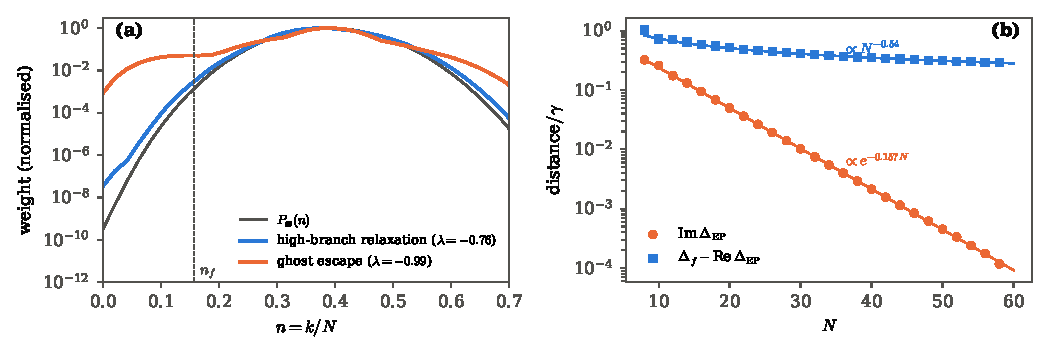
\includegraphics[width=\columnwidth]{../figs/rev_fig2.pdf}
\caption{(a) Excitation-number profiles of the two modes adjacent to the crossing ($N=48$, $\Omega=2$), with the steady-state distribution. The high-branch mode reaches the ghost region $n\approx n_f$ only through an exponentially small tail. (b) EP location: distance of ${\rm Re}\,\Delta_{\rm EP}$ from the fold (algebraic) and ${\rm Im}\,\Delta_{\rm EP}$ (exponential); lines are fits.}
\label{fig:modes}
\end{figure}

\emph{Quantum WKB theory.}---In the symmetric sector, $\Lc_N$ is a bosonic problem with $N$ quanta in four single-atom Liouville modes. Coherent-state (Doi) variables then give, for large $N$, a classical Hamiltonian $h(\hat X,\hat\rho)$. Here $\hat\rho$ is a single-atom density matrix and $\hat X$ the conjugate dual observable [Supplemental Material (SM)]:
\begin{equation}
h={\rm Re}\,{\rm Tr}\big[\hat X\,\ell_0(\hat\rho)\big]+2V\,{\rm Re}A\,{\rm Im}A,\qquad A={\rm Tr}(\hat X\hat n\hat\rho),
\label{eq:h}
\end{equation}
where $\ell_0$ is the single-atom Lindbladian at detuning $\Delta$. On the manifold $\hat X=\mathbb 1$, $h$ generates the MF flow. Fixing the gauge symmetry $(\hat\rho,\hat X)\to(\lambda\hat\rho,\hat X/\lambda)$ leaves three canonical pairs $q=(n,u,v)$, $p=(p_n,p_u,p_v)$. Here $h$ is quadratic in $p$, but its momentum Hessian is indefinite, with eigenvalues $(-a,0,a)$. Equation~\eqref{eq:h} is therefore not a Freidlin–Wentzell diffusion. Rare-event exponents are actions $\int p\,dq$ along zero-energy heteroclinics, which we obtain with Lin's method: we shoot from the unstable manifold of the high fixed point and from the target manifold, and match the two on a section (SM).

Two prerequisites validate the theory. First, the switching exponent from the high branch to the saddle agrees with the exact $s_{\rm hl}(\Delta)$, extracted from the slowest real eigenvalue of $\Lc_N$ for $N=40$--$60$, to within $0.1$--$2.8\%$ [Fig.~\ref{fig:wkb}(a)]. The result is independent of the matching section to five digits. By contrast, a Gaussian-noise minimum-action calculation overestimates $s_{\rm hl}$ by $15$--$23\%$, and an incoherent rate-equation reduction underestimates it by a factor of five. Coherences thus enter the rare-event statistics at leading order. Second, the excitation-number distribution $P(k)$ is the Fock coefficient of the Liouville bosons at occupation $x=\hat X\!\circ\!\hat\rho=(1-n,n,0,0)$, where $n=k/N$. Its rate function is the Cole–Hopf action to that occupation point,
\begin{equation}
\Phi(n)=\int p\,dq+(1-n)\ln\hat X_{gg}+n\ln\hat X_{ee}.
\label{eq:phi}
\end{equation}
On the relevant endpoint branch ($p_u=p_v=0$) the boundary term equals the Kullback–Leibler divergence $D(n\|n_{\hat\rho})$. In other words, the final step is projective counting noise. Computed without input from the exact steady state, Eq.~\eqref{eq:phi} matches the $N\to\infty$ extrapolation of $-N^{-1}\ln P(k)$ to within $0.2$--$6\%$ [Fig.~\ref{fig:wkb}(b)]. This test was pre-registered before it was computed.

\begin{figure}[t]
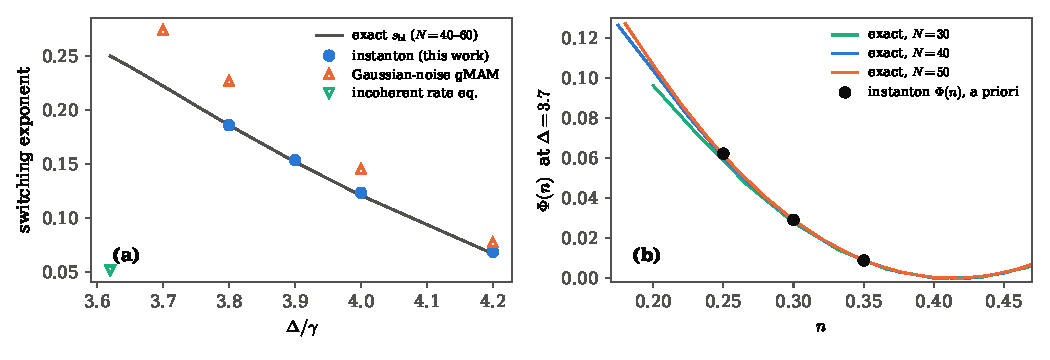
\includegraphics[width=\columnwidth]{../figs/rev_fig3.pdf}
\caption{Validation of the quantum WKB theory at $\Omega=2$. (a) Switching exponent: exact (line), quantum WKB (dots), Gaussian-noise minimum action (open triangles), incoherent rate equation (open). (b) Quasipotential of the excitation number at $\Delta=3.7$: exact finite-$N$ curves and the a-priori WKB values from Eq.~\eqref{eq:phi}.}
\label{fig:wkb}
\end{figure}

\emph{Prediction of the EP coupling.}---Figure~\ref{fig:modes}(a) suggests a simple mechanism. The ghost mode is $O(1)$ at $n_f$, whereas the high-branch mode reaches $n_f$ only through its WKB tail. Their overlap is the coupling, so
\begin{equation}
g_N\simeq c\,\exp\!\big[-N\,\Phi(n_f;\Delta_{\min}(N))\big],
\label{eq:pred}
\end{equation}
where $\Delta_{\min}(N)$ is the crossing location. We tested Eq.~\eqref{eq:pred} in two pre-registered steps on parameters not used to formulate it. Exact couplings were sealed until the predictions were frozen. (v3) With $\Phi$ read from the exact steady state at $\Omega=2.5$ and $3.0$, the fitted slopes of $\ln g_N$ vs $N\Phi$ are $0.957$ and $0.878$. The local exponents are $0.944$ and $0.878$ of the predicted values. (v4) Fully a priori, with $\Phi$ from Eq.~\eqref{eq:phi} and $\Delta_{\min}$ as the only spectral input, at $\Omega=2.25$ and $2.75$: slopes $0.958$ and $0.929$, local-exponent ratios $0.963$ and $0.934$ [Fig.~\ref{fig:pred}]. All criteria ($1\pm0.15$) passed. Two earlier registered candidates also appear in Fig.~\ref{fig:pred}(b). They used the MF fold \emph{state}, or the bottleneck hyperplane in $\hat\rho$ coordinates, and failed by factors of $2$--$4$. The endpoint must be imposed on occupations, not on density matrices. The residual $4$--$7\%$ overshoot is consistent with the missing $(\ln N)/N$ prefactor corrections, since $\Phi_{\rm WKB}$ exceeds the finite-$N$ $\Phi_N$ by $1$--$3\%$.

\begin{figure}[t]
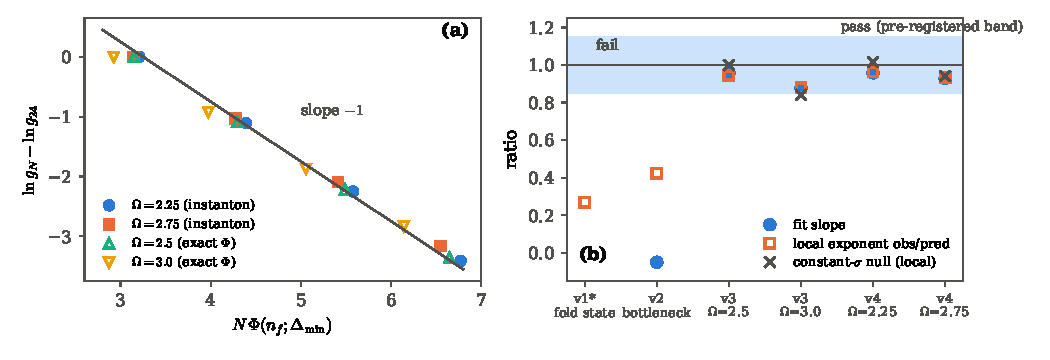
\includegraphics[width=\columnwidth]{../figs/rev_fig4.pdf}
\caption{(a) Coupling of the avoided crossing vs $N\Phi(n_f)$ at four drive strengths not used to construct Eq.~\eqref{eq:pred}. Filled: $\Phi$ from the a-priori WKB theory. Open: $\Phi$ from the exact steady state. The line has slope $-1$. (b) All pre-registered tests. v1 and v2 used other endpoint definitions and failed. v3 and v4 fall inside the registered band.}
\label{fig:pred}
\end{figure}

\emph{Consequences.}---Three consequences follow. First, the claim that a fold is an EP is correct only after a specific identification. The fold is an EP of two decaying modes of distinct physical origin, located off the real axis by an amount exponentially small in $N$ and set by a computable rate function. It is not a coalescence of steady states. Second, many-body chiral switching~\cite{Xie2025} follows a fold rule rather than an encircling rule. The final branch is set by the fold through which the bistable arc is last entered. We verified this in the published three- and four-level MF models of Ref.~\cite{Xie2025}, in which a loop that does not encircle the cusp switches (SM). In the exact dynamics the direction memory survives a loop of period $T$ with weight $\simeq\exp(-T\Lambda_N)$. Here $\Lambda_N=\int\lambda_{\rm sw}\,du$ is the switching rate integrated over the arc between the Maxwell point and the endpoint. This expression is the controlled large-$N$ limit of the exact two-state solution, which it matches to within $0.02$ at $N=40$; the two-state solution in turn agrees with full $\Lc_N$ dynamics ($N\le30$) to within $15\%$ (SM). Third, Eq.~\eqref{eq:phi} gives a practical route to rare-event exponents in collective open systems. It requires one heteroclinic in a three-degree-of-freedom phase space, not exponentially large linear algebra.

\emph{Scope.}---All statements refer to the permutation-symmetric model of Eq.~\eqref{eq:H}. Short-range interactions can replace collective switching by nucleation~\cite{Xiang2026}, and we have not addressed that case. The algebraic drift of ${\rm Re}\,\Delta_{\rm EP}$ is not yet asymptotic for $N\le58$, so we do not quote a limiting exponent for it. The crossing location $\Delta_{\min}(N)$ still enters Eq.~\eqref{eq:pred} as an exact spectral input. Pre-registration documents and all code and data are provided as SM.

\begin{thebibliography}{99}
\bibitem{Carr2013} C.~Carr, R.~Ritter, C.~G.~Wade, C.~S.~Adams, and K.~J.~Weatherill, Phys. Rev. Lett. \textbf{111}, 113901 (2013).
\bibitem{Xie2025} C.~Xie, K.~Sun, K.-D.~Wu, C.-F.~Li, G.-C.~Guo, W.~Yi, and G.-Y.~Xiang, Sci. Bull. \textbf{70}, 3345 (2025); arXiv:2402.02779.
\bibitem{Casteels2017} W.~Casteels, R.~Fazio, and C.~Ciuti, Phys. Rev. A \textbf{95}, 012128 (2017).
\bibitem{Minganti2018} F.~Minganti, A.~Biella, N.~Bartolo, and C.~Ciuti, Phys. Rev. A \textbf{98}, 042118 (2018).
\bibitem{Macieszczak2016} K.~Macieszczak, M.~Gu\c{t}\u{a}, I.~Lesanovsky, and J.~P.~Garrahan, Phys. Rev. Lett. \textbf{116}, 240404 (2016).
\bibitem{SunYi2024} K.~Sun and W.~Yi, AAPPS Bull. \textbf{34}, 22 (2024).
\bibitem{HuBudich2025} Y.-M.~Hu and J.~C.~Budich, Phys. Rev. Lett. \textbf{135}, 250402 (2025).
\bibitem{Ptaszynski2024} K.~Ptaszy\'nski and M.~Esposito, arXiv:2407.07832.
\bibitem{Xiang2026} Y.-X.~Xiang, W.~Li, Z.~Bai, and Y.-Q.~Ma, Natl. Sci. Rev. \textbf{13}, nwag146 (2026).
\bibitem{Krimer2019} D.~O.~Krimer and M.~Pletyukhov, Phys. Rev. Lett. \textbf{123}, 110604 (2019).
\bibitem{Shammah2018} N.~Shammah, S.~Ahmed, N.~Lambert, S.~De~Liberato, and F.~Nori, Phys. Rev. A \textbf{98}, 063815 (2018).
\end{thebibliography}

\end{document}
